\documentclass{article} % For LaTeX2e
\usepackage{nips11submit_e,times}
%\documentstyle[nips11submit_09,times,art10]{article} % For LaTeX 2.09

\usepackage{epsfig,subfigure}
\usepackage{amsmath,amsfonts,amssymb,amsthm}
\usepackage{array}

%\usepackage{algorithmic}
%\usepackage{algorithm}

\newtheorem{lemma}{Lemma}
\newtheorem{assumption}[lemma]{Assumption}
\newtheorem{restr}{Restriction}[section]
\newtheorem{theorem}[lemma]{Theorem}
\newtheorem{proposition}[lemma]{Proposition}
\newtheorem{corollary}[lemma]{Corollary}
\newtheorem{hypothesis}[lemma]{Hypothesis}
\newtheorem{definition}[lemma]{Definition}

\usepackage[vlined,algoruled,titlenumbered,noend]{algorithm2e}
%\usepackage{proceed2e}

\title{Exact Bayesian Pairwise Preference Learning and Inference on the Uniform Convex Polytope}
%Exact Inference on the Uniform Convex Polytope with Applications to Bayesian Preference Learning}

\author{
Scott Sanner\\
NICTA \& ANU\\
Canberra, ACT, Australia\\
\texttt{ssanner@gmail.com}
\And
Ehsan Abbasnejad\\
ANU \& NICTA\\
Canberra, ACT, Australia\\
\texttt{eabbasnejad@gmail.com}
}

% The \author macro works with any number of authors. There are two commands
% used to separate the names and addresses of multiple authors: \And and \AND.
%
% Using \And between authors leaves it to \LaTeX{} to determine where to break
% the lines. Using \AND forces a linebreak at that point. So, if \LaTeX{}
% puts 3 of 4 authors names on the first line, and the last on the second
% line, try using \AND instead of \And before the third author name.

\newcommand{\fix}{\marginpar{FIX}}
\newcommand{\new}{\marginpar{NEW}}
\newcommand{\ind}[1]{\mathbb{I}[#1]}
\newcommand{\inde}{\mathbb{I}}
\newcommand{\ie}{i.e.}

\newcommand{\var}{v}
\newcommand{\eq}{\leftarrow}

\newcommand{\LB}{\mathit{LB}}
\newcommand{\UB}{\mathit{UB}}

\newcommand{\B}{\mathbb{B}}
\newcommand{\E}{\mathbb{E}}
\newcommand{\I}{\mathbb{I}}
\newcommand{\R}{\mathbb{R}}
\newcommand{\N}{\mathcal{N}}
\newcommand{\U}{\mathcal{U}}
\newcommand{\Ind}{\mathrm{\#}}
\renewcommand{\vec}[1]{\mathbf{#1}}

\def\argmax{\operatornamewithlimits{arg\,max}}
\def\argmin{\operatornamewithlimits{arg\,min}}

\nipsfinalcopy % Uncomment for camera-ready version

\begin{document}

\maketitle

% With linear utility functions?
% Can now do PBVI with Pref. Elicitation POMDP

% Multivariate uniform often used for Bayesian utility representations
% (we could allow arbitrary polynomial functions of utility, Bayesian
%  updating still simple, argmax possible?, marginalizing constant difficult)
% (can allow GAI factors)
% - Bayesian updates from observed preferences are trivial
% - But queries not so trivial
% ** P(item_a > item_b)?  int_U I[sum_i w_i*u_i > sum_i v_i*u_i]*P(U) dU
%                         int_U I[sum_i (w_i-v_i)*u_i > 0]*P(U) dU
% ** EU[item_a] = int_U (\sum_i w_i*u_i)*P(U) dU
% ** argmax_a EU[item_a] (can then use this for max margin query)
%    would we rather do this with an LP or ILP?
% ** VOI... minimize expected loss / maximize expected improvement
% - future work: how to do argmax efficiently?  

% In Bayesian approaches to MAUT, want to learn U from preference
% observations.
% When U is uniform and preference observations lead to 
% piecewise linear likelihoods, beliefs in U represented
% as a uniform distribution on the convex polytope.
% Bayesian updating requires inferring the constant,
% other problems as well -- EU, comparison, VOI for active
% queries.  To date, MCMC sampling methods (e.g., slice sampling) 
% are most popular for inference under the general argument that 
% the exact solution (equivalent to computing the volume of
% a convex polytope) is intractable (SAT is intractable too,
% the real issue here is that there is no off-the-shelf code
% for computing such volumes).

% Bayesian Utility 
% Math
% Solution with cases
% Empirical results

\begin{abstract}
In Bayesian approaches to utility learning from preferences, the
objective is to infer a posterior belief distribution over an agent's
utility function based on previously observed agent preferences.  From
this, one can then estimate quantities such as the expected utility of
a decision or the probability of an unobserved preference,
%, or even the value of
%information of an additional preference query w.r.t.\ the posterior
%utility beliefs for the agent.
which can then be used to make or suggest future decisions on behalf
of the agent.  However, there remains an open question as to how one
can represent beliefs over agent utilities, perform Bayesian updating
based on observed agent \emph{pairwise} preferences, and make
inferences with this posterior distribution in an exact, closed-form.
In this paper, we build on Bayesian pairwise preference learning
models under the assumptions of linearly 
%(generalized) 
additive multi-attribute utility functions and a bounded uniform
utility prior.  These assumptions lead to a posterior form that is a
uniform distribution over a convex polytope for which we then
demonstrate how to perform \emph{exact, closed-form} inference w.r.t.\
this posterior, i.e., without resorting to sampling or
other approximation methods.
\end{abstract}
% Note also applies to learning from Bayesian ranking

\section{Introduction}

\label{sec:intro}

Decision support systems (DSSs) require knowledge of an agent's
preferences in order to make or suggest future decisions on their
behalf.  Clearly then, the most crucial task of a DSS is in learning to
predict future agent preferences from previously observed agent preferences.

In recent years, an increasingly popular approach to preference
learning relies on Bayesian updating of posterior beliefs in an
underlying (multi-attribute) utility function conditioned on observed
agent
preferences~\cite{Chajewska00utilitiesas,Chajewska01learningan,boutilier02239,zoubin_gp,sanner:aistats10,viappiani_nips};
inference can then be performed by marginalizing over these posterior
utility beliefs w.r.t.\ future preference queries.  This \emph{Bayesian
preference learning} (BPL) is attractive for a multitude of reasons,
among them (a) the generally acknowledged robustness of Bayesian
learning methods to overfitting, (b) the fact that updates can be done
online, and (c) the fact that Bayesian methods provide a useful
measure of confidence in their predictions via a probability
distribution over predicted outcomes.

Despite the attractiveness of BPL, we are not aware of a Bayesian
\emph{pairwise} preference learning (BPPL) approach that claims to do
all learning and inference in an exact, closed-form.  Arguably the two
most common priors for BPPL are either Gaussian or Uniform --- in the
former case, a Gaussian prior is not conjugate to commonly used
pairwise preference likelihoods leading to the need for approximate
Bayesian updating in order to maintain a tractable form for the
posterior~\cite{Chajewska00utilitiesas,boutilier02239,zoubin_gp,sanner:aistats10}, in
the latter case, certain Uniform distributions are indeed conjugate to
commonly used pairwise preference likelihoods, \emph{but} inference
with the posterior convex polytope requires difficult integrals 
%inference that is 
%$\sharp$P-Complete (poly-time only if P=NP) and is thus 
that in practice are approximated via sampling or other
methods~\cite{Chajewska01learningan,viappiani_nips}.

In this paper, we argue that the exact integrals in the case of BPPL
with commonly used linearly additive multi-attribute utility functions
and a uniform utility prior are not as computationally difficult as
they may appear.  Indeed, armed with symbolic inference for piecewise
functions and efficient data structures derived from algebraic
decision diagram (ADD) for representing and performing operations on
these functions, we show that such inference can be computed
efficiently for reasonably sized problems in practice.
%exact inference which is $\sharp$P-Complete
%is not as bad it may sound considering that satisfiability is an NP-Complete
%problem, but yet can be solved for extremely large instances.
This is the first time (to the best of the authors' knowledge) that an
explicit algorithm has been provided for doing BPPL and all associated
inference in exact, closed-form.

\section{Bayesian Pairwise Preference Learning (BPPL)}

Here we follow much of the BPPL setup of~\cite{sanner:aistats10},
except for the case of a Uniform rather than Gaussian prior distribution.  
In \emph{multi-attribute
utility theory} (MAUT)~\cite{keeney_raiffa76}, utilities are modeled
over a $D$-dimensional \emph{attribute vector} $\vec{x}$ where each
\emph{attribute choice} $x_d$ ($1 \leq d \leq D$) is either binary
($x_d \in \{0 \mbox{ (false)},1 \mbox{ (true)}\}$) or real-valued
($x_d \in \R$).  An \emph{item} is described by its attribute choice
assignments $\vec{x}=(x_{1},\dots,x_{D})$.  For example, let our
item space consist of possible cars we might buy, let binary attribute
choice $x_1$ represent whether the car is a \emph{2-door} (if false,
we assume it is a \emph{4-door}) and let $x_2$ represent the amount of
\emph{engine displacement in liters}.  Perhaps two of our available
items are a 2.4L two-door Accord with attribute vector $\vec{x}^a =
(1,2.4)$ and a 3.5L four-door Buick with attribute vector $\vec{x}^b =
(0,3.5)$.

Our goal in BPPL will be to learn an \emph{attribute weight vector}
$\vec{w} = \mathbb{R}^D$ that describes the utility of \emph{each}
attribute choice in \emph{each} attribute dimension.  As commonly done
in MAUT~\cite{keeney_raiffa76,bacchus_grove}, we assume that the overall 
utility $u(\vec{x}|\vec{w})$ of item $\vec{x}$ w.r.t.\ attribute
weight vector $\vec{w}$ decomposes \emph{additively} over the
attribute choices of $\vec{x}$, i.e.,
\begin{equation}\label{eq:util}
u(\vec{x}|\vec{w}) = \sum_{d=1}^{D} \vec{w}_d \vec{x}_d .
\end{equation}

We let $u^*$ represent the user's true utility w.r.t.\ their true (but
hidden) $\vec{w}^*$.  Since $\vec{w}^{*}$ is unknown to the decision
support system, we take a Bayesian perspective on learning
$\vec{w}$~\cite{Chajewska00utilitiesas} and thus maintain a
probability distribution $P(\vec{w})$ representing our beliefs over
$\vec{w}^{*}$.  For this, we must define our prior utility beliefs,
likelihood (preference query response model), the form of
the posterior for our Bayesian update, and the form of any inferences
we wish to make with the posterior.

\subsection{Utility Prior}

For our prior beliefs $P(\vec{w})$, we start with a hyper-rectangular
multivariate uniform distribution over $\vec{w}$ represented
as follows
\begin{equation} \label{eq:prior}
P(\vec{w}) = \prod_{d=1}^{D} p(w_{d})
           = \prod_{d=1}^{D} \U(w_{d};-C,C).
\end{equation}
where $C \in \R$ ($C \neq 0$) is some constant~\footnote{In
practice, $C$ could be different for each dimension, if justified.}
and the uniform distribution $\U$ is simply defined using an indicator
function\footnote{We use $\I[\cdot]$ as an indicator function taking
the value $1$ when its argument is true and $0$ otherwise.}:
\begin{align*}
\U(w_d;L,U) & = \frac{1}{U-L} \I[(w_d \geq L) \land (w_d \leq U)].
\end{align*}
By using respective lower and upper bounds of
$-C$ and $C$ for each uniform dimension of the prior, we enforce that
$\E_{\vec{w} \sim P(\vec{w})}[\vec{w}] = \vec{0}$ indicating agnostic
prior beliefs about the utility of each attribute.  

As it will be important observation for future sections, we remark
that such a hyperrectangular uniform prior as defined here can also be
conveniently viewed as the intersection (product) of half-spaces given
by the indicator definition of $\U$.

\subsection{Query \& User Response Model}

\label{sec:query_and_user_model}

In this paper, we focus on pairwise comparison queries known to
require low cognitive load for users to answer~\cite{conitzer09161}.
We use $Q_{ab} = \{ a \succ b, a \prec b, a \sim b \}$ to represent a
pairwise comparison query indicating the user's preferences of item
$\vec{x}^a$ vs. item $\vec{x}^b$ (henceforth just $a$ and $b$).
Depending on the user's attribute weight vector $\vec{w}$ and the
corresponding item utilities, $u(a|\vec{w})$ and $u(b|\vec{w})$, the
user's response $q_{ab} \in Q_{ab}$ indicates the following:
\begin{itemize}
\item $a \succ b$: the user prefers $a$ to $b$,
\item $a \prec b$: the user prefers $a$ to $b$,
\item $a \sim b$:  the user is indifferent between $a$ and $b$.
\end{itemize}

We represent the user query model in
(\ref{eq:bayes_update}) with an indicator function over the pairwise utility
differences as follows 
\begin{align}
P(Q_{ab}=a \succ b|\vec{w}) & \; = \; \I[u(a|\vec{w}) - u(b|\vec{w}) > \epsilon] \nonumber \\
P(Q_{ab}=a \prec b|\vec{w}) & \; = \; \I[u(b|\vec{w}) - u(a|\vec{w}) > \epsilon] \nonumber \\
P(Q_{ab}=a \sim  b|\vec{w}) & \; = \; \I[|u(a|\vec{w}) - u(b|\vec{w})| \leq \epsilon], 
\label{eq:p_qij_hat}
\end{align}
where we can modulate the range of utility differences for which the
user is indifferent by adjusting $\epsilon$.  Note that by definition,
$\sum_{q_{ab}} P(q_{ab}|\vec{w}) = 1$.

If needed, we could easily model more noise in the elicitation process
simply by allowing non-zero probability for weight vectors that
disagree with the query response.  For example, here we model a 10\%
chance that a user's query response disagrees with their utility valuation
of items $a$ and $b$ by more than $\epsilon$:
\begin{align}
P(Q_{ab}=a \succ b|\vec{w}) & \; = \; 0.9 \cdot \I[u(a|\vec{w}) - u(b|\vec{w}) > \epsilon]  + 0.1 \cdot \I[u(a|\vec{w}) - u(b|\vec{w})] \leq \epsilon \label{eq:p_qij_mod} .
\end{align} 
Whatever exact form of the above query response model is used, we note
that due to the linearity of $u(\cdot|\vec{w})$ in $\vec{w}$, all of
the above query response likelihood models can be represented by (a
sum of) linearly separated half-spaces owing to the the linear
constraints in the likelihood indicator functions.

\subsection{Bayesian Utility Updating}

\label{sec:pe_model_infer}

Given a prior utility belief $P(\vec{w}|R^n)$ w.r.t.\ a
(possibly empty) set of $n \geq 0$ query responses $R^n = \{ q_{kl}
\}$ and a new query response $q_{ab}$, we perform the following
Bayesian update to obtain a posterior belief $P(\vec{w}|R^{n+1})$
where $R^{n+1} = R^n \cup \{ q_{ab} \}$:
\begin{align}
P(\vec{w}|R^{n+1}) & \propto P(q_{ab}|\vec{w},R^n) P(\vec{w}|R^n) \nonumber \\
                   & \propto P(q_{ab}|\vec{w}) P(\vec{w}|R^n). \label{eq:bayes_update}
\end{align}
Assuming that our query likelihood $P(q_{ab}|\vec{w})$ is modeled as
described in~\eqref{eq:p_qij_hat} [or~\eqref{eq:p_qij_mod}], we note
that since the prior is a product of linear half-spaces and the
likelihood also [a sum of] linear half-spaces and these are
multiplied, the resulting posterior is a \emph{uniform convex
polytope}\footnote{Here an unnormalized uniform distribution on the
convex polytope defined by the product of linear constraints in the
indicator functions.} [or after placing the result in sum of products
form, a sum of uniform convex polytopes].  Hence, an unnormalized
Bayesian update appears to be computationally straightforward --- 
and in fact a 
very efficient $O(nD)$ complexity for Bayesian updating 
for the case of the likelihood model in~\eqref{eq:p_qij_hat}.

In Figure~\ref{fig:polytope}, we show a $D=2$ representation of a
posterior for a likelihood in the form of~\eqref{eq:p_qij_hat}

%%%%%%%%%%%%%%%%%%%%%%%%%%%%%%%%%%%%%%%%%%%%%%%%%%%%%%%%%%%%%%%%%%%%%%%%%%
\begin{figure}[t!]
\begin{center}
\vspace{-1mm}
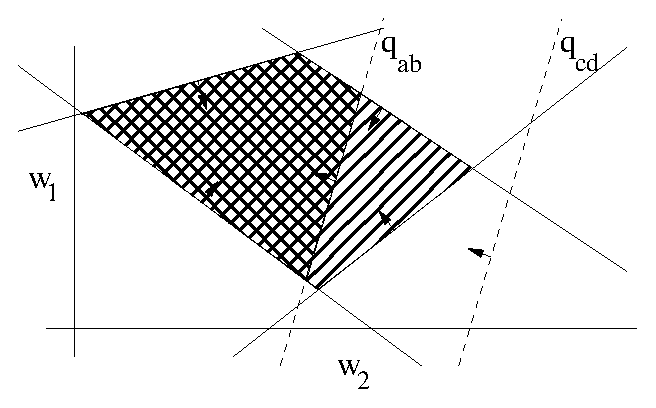
\includegraphics[width=.6\textwidth]{polytope}
\end{center}
\vspace{-4mm}
\caption{\footnotesize A representation of the uniform convex polytope
representing the posterior distribution on $\vec{w}$ when using the
likelihood model in~\eqref{eq:p_qij_hat}.  The union of the 
striped and cross-hatched area shows 
the non-zero posterior polytope before updating with query response
$q_{ab}$ and the cross-hatched area shows the non-zero posterior
polytope after updating with query response $q_{ab}$.  We note that
query response $q_{cd}$ would not lead to any change in either 
posterior before or after updating with $q_{cd}$ and its constraint
could be pruned from the constraint set.} \label{fig:polytope}
\end{figure}
%%%%%%%%%%%%%%%%%%%%%%%%%%%%%%%%%%%%%%%%%%%%%%%%%%%%%%%%%%%%%%%%%%%%%%%%%%

\subsection{Preference Inference}

\label{sec:bppl_inference}

% ** P(item_a > item_b)?  int_U I[sum_i w_i*u_i > sum_i v_i*u_i]*P(U) dU
%                         int_U I[sum_i (w_i-v_i)*u_i > 0]*P(U) dU
% ** EU[item_a] = int_U (\sum_i w_i*u_i)*P(U) dU

Now that we have posterior beliefs in our utility weighting 
$P(\vec{w}|R^n)$, we would like to perform at least two types of inference:
\begin{itemize}
\item {\it Item with maximum expected utility:} 
\begin{align*}
& \argmax_{\vec{x}} \; \E_{\vec{w}} \left[ u(\vec{x}|\vec{w}) \big| R^n \right]\\ & = \argmax_{\vec{x}} \int_{\vec{w}} P(\vec{w}|R^n) \left[ \sum_{d=1}^{D} \vec{w}_d \vec{x}_d \right] d\vec{w}
\end{align*}
\item {\it Probability of preference outcomes:} 
\begin{align*}
P(q_{ab} | R^n) \; & = \int_\vec{w} P(q_{ab} | \vec{w}) P(\vec{w}|R^n) d\vec{w}
\end{align*}
\end{itemize}
If using likelihood form~\eqref{eq:p_qij_hat}, we note that both
inferences are volume integrals over a function ($u(\vec{x}|\vec{w})$
in the first case and constant in the latter case) subject to boundary
constraints over a convex polytope defined w.r.t.\ $P(\vec{w}|R^n)$
(appearing in both inferences) and $P(q_{ab} | \vec{w})$ (only for the
second inference).  In the case of likelihood
form~\eqref{eq:p_qij_hat}, we simply get a sum of such integrals.
Consequently, the question we have to ask to perform exact inference
in this Uniform BPPL setting is the following: given a function
defined over the region of a convex polytope like the one in
Figure~\ref{fig:polytope}, how do we compute this integral in
closed-form?

At first, this would seem quite difficult --- the boundaries in any
dimension in Figure~\ref{fig:polytope} may be a piecewise function of
the other dimensions --- but on closer inspection, there is a
systematic way to compute these integrals if given the right
representation.  We discuss this next.

\section{Symbolic Variable Elimination in Discrete/Continuous Graphical Models}

In this section, we introduce a \emph{case} notation and operations
for piecewise polynomial functions and demonstrate that all Uniform
BPPL operations, including the required integrals can be computed
exactly and in closed-form using a purely \emph{symbolic}
representation.

\subsection{Case Representation and Operators}

For this section, we will assume all functions
are represented in \emph{case} form~\cite{uai11} as follows:
{%\footnotesize 
\begin{align}
f = 
\begin{cases}
  \phi_1 & f_1 \\ 
  \vdots & \vdots \\ 
  \phi_k & f_k \\ 
\end{cases} \label{eq:case}
\end{align}
} Here, the $f_i$ may be \emph{polynomial} functions of $\vec{w}$ (although
initially the functions $f_i$ will be constant or linear, we will see
that integration will introduce higher order polynomials for $f_i$).  The
$\phi_i$ are logical formulae defined over $\vec{w}$ that can consist
of arbitrary logical combinations of inequalities ($\geq,>,\leq,<$)
over \emph{linear} functions of $\vec{w}$.  We assume that the set of
conditions $\{ \phi_1,\ldots,\phi_k \}$ disjointly and exhaustively
partition $\vec{w}$ such that $f$ is well-defined for all $\vec{w} \in
\R^D$.  It is easy to verify that such a representation can represent
all of the functions discussed in Section~\ref{sec:pe_model_infer}.

\emph{Unary operations} such as scalar multiplication $c\cdot f$ (for
some constant $c \in \mathbb{R}$) or negation $-f$ on case statements
$f$ are straightforward; the unary operation is simply applied to each
$f_i$ ($1 \leq i \leq k$). Intuitively, to perform a \emph{binary
  operation} on two case statements, we simply take the cross-product
of the logical partitions of each case statement and perform the
corresponding operation on the resulting paired partitions.  Thus, we 
perform the ``cross-sum'' $\oplus$ of two (unnamed) cases as follows:
{\footnotesize 
\begin{center}
\begin{tabular}{r c c c l}
&
\hspace{-6mm} 
  $\begin{cases}
    \phi_1: & f_1 \\ 
    \phi_2: & f_2 \\ 
  \end{cases}$
$\oplus$
&
\hspace{-4mm}
  $\begin{cases}
    \psi_1: & g_1 \\ 
    \psi_2: & g_2 \\ 
  \end{cases}$
&
\hspace{-2mm} 
$ = $
&
\hspace{-2mm}
  $\begin{cases}
  \phi_1 \wedge \psi_1: & f_1 + g_1 \\ 
  \phi_1 \wedge \psi_2: & f_1 + g_2 \\ 
  \phi_2 \wedge \psi_1: & f_2 + g_1 \\ 
  \phi_2 \wedge \psi_2: & f_2 + g_2 \\ 
  \end{cases}$
\end{tabular}
\end{center}
}
\normalsize
Likewise, we perform $\ominus$ and $\otimes$ by,
respectively, subtracting or multiplying partition values (rather than
adding them) to obtain the result.  
%Clearly the decisions remain logical combinations of linear
%inequalities and the functions remain polynomials.
%If the operands are well-defined functions then it is easy to see
%the result will be as well.
Some partitions resulting from
the application of the $\oplus$, $\ominus$, and $\otimes$ operators
may be inconsistent (infeasible); if we can detect this (e.g., via
a linear constraint solver), we may simply discard such 
partitions as they are irrelevant to the function value.

For the Uniform BPPL inference defined in
Section~\ref{sec:bppl_inference}, we'll need to compute definite
integrals --- a fairly non-trivial operation that is discussed in its
own section.  But first we discuss maximization needed for working
with integral bounds.

\emph{Symbolic maximization} is fairly straightforward
to define:
%\vspace{-5mm}

{\footnotesize
\begin{center}
\begin{tabular}{r c c c l}
&
\hspace{-9mm} $\max \Bigg(
  \begin{cases}
    \phi_1: & f_1 \\ 
    \phi_2: & f_2 \\ 
  \end{cases}$
$,$
&
\hspace{-4mm}
  $\begin{cases}
    \psi_1: & g_1 \\ 
    \psi_2: & g_2 \\ 
  \end{cases} \Bigg)$
&
\hspace{-4mm} 
$ = $
&
\hspace{-4mm}
  $\begin{cases}
  \phi_1 \wedge \psi_1 \wedge f_1 > g_1    : & f_1 \\ 
  \phi_1 \wedge \psi_1 \wedge f_1 \leq g_1 : & g_1 \\ 
  \phi_1 \wedge \psi_2 \wedge f_1 > g_2    : & f_1 \\ 
  \phi_1 \wedge \psi_2 \wedge f_1 \leq g_2 : & g_2 \\ 
  \phi_2 \wedge \psi_1 \wedge f_2 > g_1    : & f_2 \\ 
  \phi_2 \wedge \psi_1 \wedge f_2 \leq g_1 : & g_1 \\ 
  \phi_2 \wedge \psi_2 \wedge f_2 > g_2    : & f_2 \\ 
  \phi_2 \wedge \psi_2 \wedge f_2 \leq g_2 : & g_2 \\ 
  \end{cases}$
\end{tabular}
\end{center}
}
% Need to note that max can be problematic as it could introduce
% polynomial constraints... have to guarantee this does not occur...
% occur here (max only over constraint parts) and in SVE with
% linear constraints... I think SVE with nonlinear constraints
% cannot always be computed as in SVE since the nonlinear constraints
% hang around until the variable is eliminated.  Also a problem for
% decision making with actions and noise (e.g., Utility diagrams, MDPs,
% POMDPs) because nonlinear value functions introduce nonlinear
% constraints and integration is needed later... but integration is
% only needed over noise variables... I guess as long as these
% occur linearly, then things are OK?
The key observation here is that case statements are closed under the
max operation.  While it may appear that this representation will lead
to an unreasonable blowup in size, we note the XADD that we introduce
later in Section~\ref{sec:xadd} will be able to exploit the internal
decision structure of this maximization to represent it much more
compactly.

\subsection{Integration on the Convex Polytope}

\label{sec:def_int}

We have almost all of the operations needed to perform Uniform BPPL
inference as defined in Section~\ref{sec:bppl_inference}, except for a
method to compute each of the integrals $\int_{w_1},\ldots,\int_{w_D}$
w.r.t. the convex polytope constraints such as those shown in
Figure~\ref{fig:polytope}.  We provide this integration technique
here.

If we are computing $\int_{w_1=-\infty}^{\infty} f \, dw_1$ for $f$
in~\eqref{eq:case}, we can rewrite it in the following equivalent form
\begin{equation}
\int_{w_1=-\infty}^{\infty} \sum_i \I[\phi_i] \cdot f_i \, dw_1 \; = \; \sum_i \int_{w_1=-\infty}^{\infty} \I[\phi_i] \cdot f_i \, dw_1 . \label{eq:int_decomp}
\end{equation}
Hence we can compute the integrals separately for each case partition
(producing a case statement) and then $\sum$ the results using
$\oplus$.

To continue with the integral for a single case partition, we
introduce a concrete example.  Let $f_1 := 3 w_1 - 2 w_2$ and $\phi_1
:= [w_1 > -1] \land [w_1 > w_2-1] \land [w_1 \leq -w_2] \land [w_1 \leq w_2 +1] \land [w_2 > 0]$.  
In computing $\int_{w_1=-\infty}^{\infty} \I[\phi_1] \cdot f_1 \, dw_1$,
the first thing we note is that the constraints involving $w_1$ in
$\I[\phi_1]$ can be used to restrict the integration range for $w_1$.
In fact, we know that the integrand is only non-zero for
$\max(w_2 - 1, -1) \leq w_1 \leq \min(-w_2,w_2 + 1)$.  Using the $\max$
and corresponding $\min$ operations defined previously, let us 
write explicit functions for these bounds in 
\emph{piecewise linear case form} for the respective 
lower and upper bounds $\LB$ and $\UB$:
{\footnotesize
\begin{center}
\begin{tabular}{r c c l}
&
\hspace{-6mm} 
  $\LB := \begin{cases}
    w_2 - 1 > -1: & w_2 - 1 \\ 
    w_2 - 1 \leq -1: & -1 \\ 
  \end{cases}$
&

&
\hspace{-2mm}
  $\UB := \begin{cases}
    -w_2 < w_2 + 1 : & -w_2 \\ 
    -w_2 \geq w_2 + 1 : & w_2 + 1 \\ 
  \end{cases} = 
  \begin{cases}
    w_2 \geq -\frac{1}{2} : & -w_2 \\ 
    w_2 < -\frac{1}{2} : & w_2 + 1 \\ 
  \end{cases}$
\end{tabular}
\end{center}
}
Now we can rewrite the integral as\footnote{The careful reader will note
that because the lower bounds were defined in terms of $>$
rather than $\leq$, we technically have an improper integral
and need to take a limit.  However, in taking the limit, we
note that all integrands are continuous polynomials
of order 0 or greater, so the limit exists and yields the
same answer as substituting the limit value.  Hence for 
polynomials, we need not be concerned about whether bounds
are inclusive or not.}
\begin{equation}
\I[w_2 > 0] \int_{w_1=\LB}^{\UB} (3 w_1 - 2 w_2) \, dw_1 .
\end{equation}
Note here that $\I[w_2 > 0]$ is independent of $w_1$ and hence
can factor outside the integral.  With all indicator functions
moved into the $\LB$ or $\UB$ or factored out, we can now compute
the integral:
\begin{equation}
\I[w_2 > 0] \left[ \frac{3}{2}w_1^2 - 2 w_2 w_1 \bigg|_{w_1=\LB}^{w_1=\UB} \right] .
\end{equation}
The question now is simply how to do this evaluation?  Here we note
that every expression (variables, constants, indicator functions, etc.) 
can be written as a 
simple case statements or as operations on case statements, even the upper
and lower bounds as shown previously.  So the evaluation is simply:
{\footnotesize
\begin{align}
 & \I[w_2 > 0] \otimes \left[ \frac{3}{2} \UB \otimes \UB \ominus \fbox{$2 w_2$} \otimes \UB \right] \ominus \left[ \frac{3}{2} \LB \otimes \LB \ominus \fbox{$2 w_2$} \otimes \LB \right] \label{eq:almost_final}
\end{align}}
Hence the result of the definite integration over a case
partition of a polynomial function with piecewise linear constraints
is a case statement with piecewise linear constraints over polynomial
functions --- this is somewhat remarkable given that
all of the bound computations were symbolic.  

However, we are not yet done, there is one final step that we must
include for correctness.  Because our bounds are symbolic, it may be
the case for some assignment to $(\vec{b},\vec{w})$ that $\LB \geq
\UB$ (this occurs in infeasible portions of the convex polytope).  
In this case the integral should be zero since the constaints
on $w_1$ could not be jointly satisfied.  To enforce this
symbolically, we simply need to $\otimes$~\eqref{eq:almost_final} by
case statements representing the following inequalities for all pairs
of upper and lower bounds:
\begin{equation}
\I[-w_2 > w_2 - 1] \otimes \I[-w_2 > -1] \otimes \I[w_2 + 1 > w_2 - 1] \otimes \I[w_2 + 1 > -1]
\end{equation}
Of course, here $\I[w_2 + 1 > w_2 - 1]$ could be removed as a tautology,
but not the other constraints.

This provides the solution for a single case partition and 
from~\eqref{eq:int_decomp}, we just need to $\oplus$ the case
statements from each case partition integral evaluation to obtain
the full integral, still in case form.  Repeating this for all integrals
$\int_{w_1},\ldots,\int_{w_D}$, we can obtain closed-form exact results
for all queries in Section~\ref{sec:bppl_inference}!

%%%%%%%%%%%%%%%%%%%%%%%%%%%%%%%%%%%%%%%%%%%%%%%%%%%%%%%%%%%%%%%%%%%%%%%%%%
\begin{figure*}[t!]
\begin{center}
\begin{tabular}{m{.70\textwidth}m{.03\textwidth}m{.25\textwidth}}
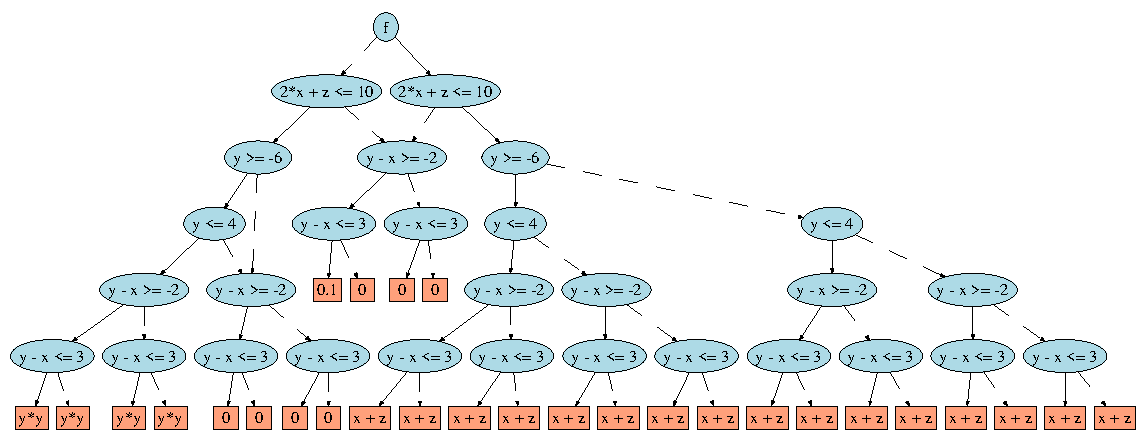
\includegraphics[width=.70\textwidth]{norm_unif_tree}  & 
\vspace{-.8cm} \hspace{-7mm} \large $\underrightarrow{\qquad}$ & 
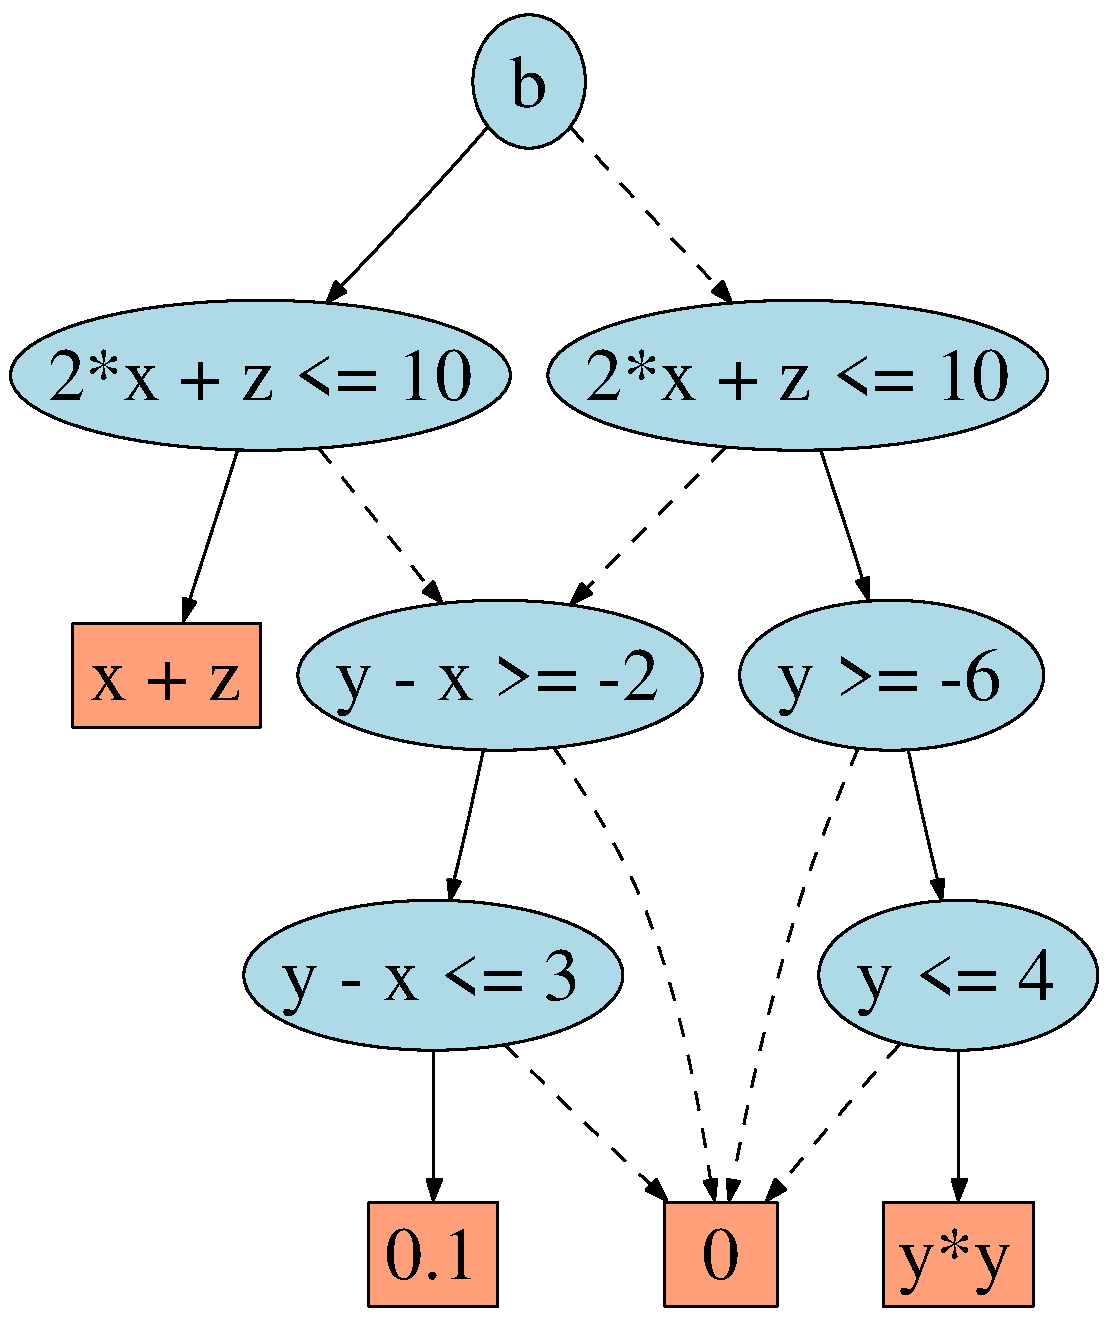
\includegraphics[width=.20\textwidth]{norm_unif}
\end{tabular}

\end{center}
\caption{\footnotesize {\it Left:} a tree representation of a case statement: each branch corresponds to a single case partition.  {\it Right:} minimal XADD
representation of the same case statement, note the compact DAG 
structure.} \label{fig:xadd_tree}
\end{figure*}
%%%%%%%%%%%%%%%%%%%%%%%%%%%%%%%%%%%%%%%%%%%%%%%%%%%%%%%%%%%%%%%%%%%%%%%%%%

\section{Extended ADDs (XADDs) for Case Statements}

\label{sec:xadd}

In practice, it can be prohibitively expensive to maintain a case
statement representation of a value function with explicit partitions.
Motivated by algebraic decision diagrams (ADDs)~\cite{bahar93add},
which maintain compact representations for finite discrete functions,
we use an extended ADD (XADD) formalism introduced 
in~\cite{uai11} and demonstrated in 
Figure~\ref{fig:xadd_tree} (right).

In brief we note that an XADD is like an algebraic decision 
diagram (ADD)~\cite{bahar93add} except that (a) the decision
nodes can have arbitrary inequalities, equalities, or disequalities (one
per node) and (b) the leaf nodes can represent arbitrary functions.
The decision nodes still have a fixed order from root to leaf
and the standard ADD
operations to build a canonical ADD (\textsc{Reduce}) and 
to perform a binary operation on two ADDs (\textsc{Apply}) 
still applies in the case of XADDs. 

Of particular importance is that the XADD is a directed acyclic graph
(DAG), and hence is often much more compact than a tree
representation.  For example, in Figure~\ref{fig:xadd_tree} (left) we provide
the function represented by the XADD in Figure~\ref{fig:xadd_tree} (right) 
expanded from a DAG into it's full tree form.  We note that not only is
the XADD much more compact on account of its DAG, but that all
unary and binary operations on XADDs can directly exploit this
compact structure for efficiency.  For more compactness and hence efficiency, 
we can apply a linear
constraint solver to prune out unreachable branches of the convex
polytope so that for example, dominated polytope constraints 
for preference $q_{cd}$ in Figure~\ref{fig:polytope} can simply
be pruned from the XADD.

To this end, we can use the XADD to perform all case operations
required for inference in Section~\ref{sec:pe_model_infer} and hence
efficiently perform the Uniform BPPL queries from
Section~\ref{sec:bppl_inference} as we demonstrate next.

\section{Empirical Results}

%%%%%%%%%%%%%%%%%%%%%%%%%%%%%%%%%%%%%%%%%%%%%%%%%%%%%%%%%%%%%
\begin{figure}[t!]
\centering
\vspace{-40mm}
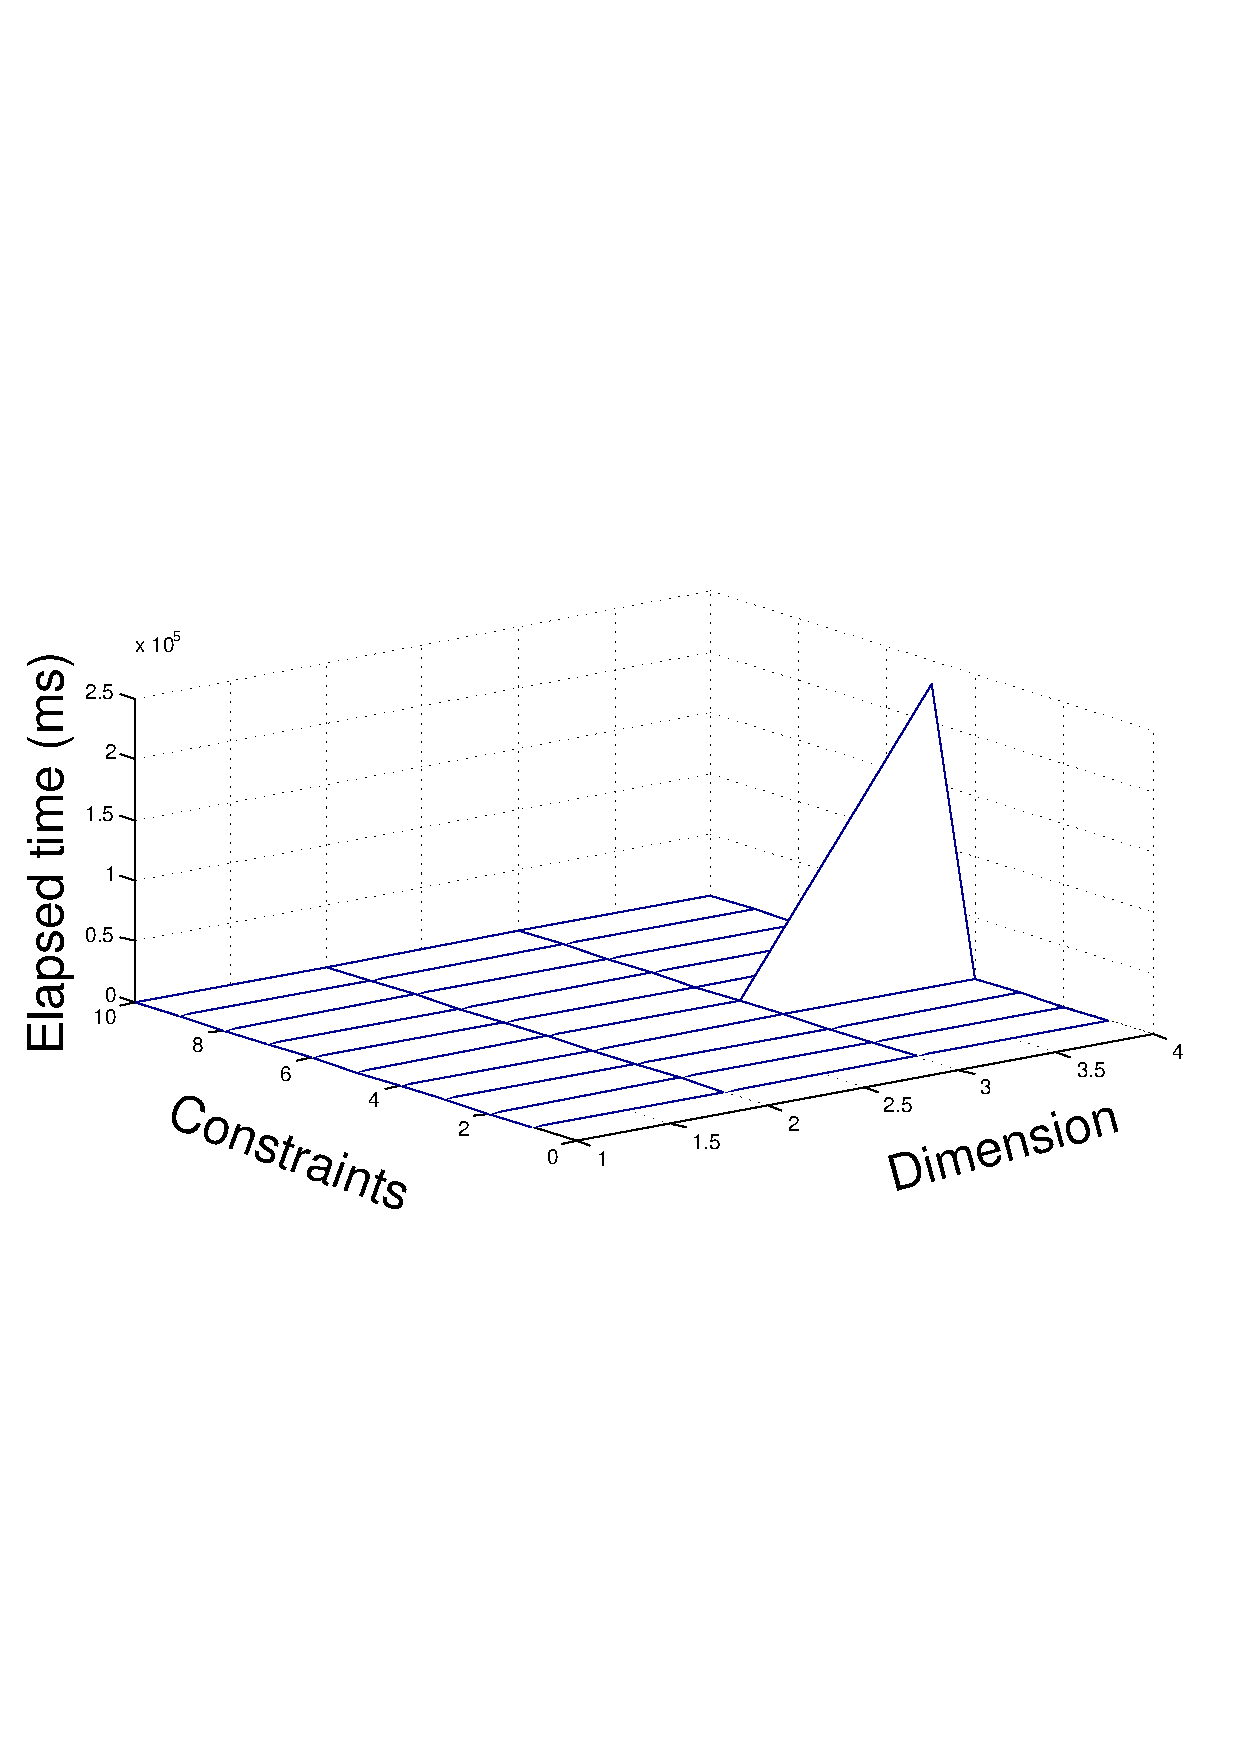
\includegraphics[width=.6\textwidth,clip=true]{dim_constraint_time}
\vspace{-35mm}
\caption{\footnotesize
The performance of expected utility computation of~\eqref{eq:expected_utility} in terms of time in ms with various dimensionality (utility attributes) and number of constraints (query responses).} \label{fig:running_time}
\end{figure}
%%%%%%%%%%%%%%%%%%%%%%%%%%%%%%%%%%%%%%%%%%%%%%%%%%%%%%%%%%%%%

In this section we demonstrate that performing the inference from
Section~\ref{sec:bppl_inference} is efficient in most cases for
a reasonable number of attribute dimensions and pairwise query
response observations.

In Figure~\ref{fig:running_time}, we illustrate how the algorithm
performs as the number of attributes $D$ (i.e., dimensionality) 
and the size ($n$) of the query response set $R^n$ 
(i.e., number of constraints) vary.
To run this experiment, we randomly generated an attribute weighting
vector $\vec{w}$ of dimensionality $D$ as well as 
$n$ query responses $R^n$
(ensuring all responses maintained a feasible utility region),
performed Bayesian updating under the likelihood model 
of~\eqref{eq:p_qij_hat}, 
and then carried out the expected utility
sub-query from Section~\ref{sec:bppl_inference}:
\begin{align}
\E_{\vec{w}} \left[ u(\vec{x}|\vec{w}) \big| R^n \right] = \argmax_{\vec{x}} \int_{\vec{w}} P(\vec{w}|R^n) \left[ \sum_{d=1}^{D} \vec{w}_d \vec{x}_d \right] d\vec{w} \label{eq:expected_utility}
\end{align}
We recorded the total time of this inference as a function of the
dimensionality $D$ and number of constraints $n$.

As we can observe in Figure~\ref{fig:running_time}, in general the
expected utility inference runs within a reasonable time for most
cases (the flat surface is not zero, but rather on the order of 100 ms
or less).  Curiously, it is only for a certain combination of
constraints and dimensionality that the algorithm fails to run fast
enough for real-time performance --- empirically, it seems that
over-constrained and under-constrained problems for lower dimensions
are easiest for inference.  It remains to explain exactly why this
happens --- intuitively, one would have thought the smaller the number
of constaints, the easier the piecewise integrals can be evaluated.
We are currently investigating this phenomena in more detail.

\section{Conclusions and Future Work}

This work presented novel and efficient, exact Bayesian learning and
inference methods for preference elicitation on the Uniform
distribution on the convex polytope.  In future work, we aim to
investigate the following possible extensions:
\begin{itemize}
\item {\it Generalized additive
independence}~\cite{keeney_raiffa76,bacchus_grove}: can we introduce additive
independence over joint utility factors rather than individual utility 
attributes while still achieving efficient computation?  In principle,
this seems relatively straightforward.
\item {\it Nonlinear utility functions}: under what conditions can we
use nonlinear utility functions and still compute the inferences from
Section~\ref{sec:bppl_inference}?
\item {\it Multi-user utility inference}: how can we extend the
inference in this paper to leverage query responses from multiple
users in a Bayesian \emph{collaborative filtering}~\cite{collab_filtering} 
framework?
\end{itemize}

\section*{Acknowledgements}

NICTA is funded by the Australian Government as represented by
the Department of Broadband, Communications and the Digital
Economy and the Australian Research Council through the ICT
Centre of Excellence program.

\bibliographystyle{plain}

\end{document}
